\documentclass[a4paper,11pt]{article}
\usepackage{anysize}
\marginsize{3cm}{2cm}{1cm}{1cm}
\usepackage[polish]{babel}
\usepackage[OT1]{fontenc}
\usepackage[utf8]{inputenc}
\usepackage{titlesec}
\usepackage[table]{xcolor}
\usepackage{graphicx}
\usepackage{multirow}% (1) choose a font that is available as T1
% for example:
\usepackage{lmodern}
\usepackage{listings}
\usepackage{hyperref}

% (2) specify encoding
\usepackage[T1]{fontenc}

% (3) load symbol definitions
\usepackage{textcomp}

\titlelabel{\thetitle.\quad}
\title{\mbox{\textbf{Laboratorium Optymalizacji Kombinatorycznej}}\newline\newline
Algorytm heurystyczny dla problemu Job-Shop Scheduling\\
\Large{Prowadzący: prof. dr hab. inż. Maciej Drozdowski}}
\author{Krzysztof Marciniak - 106574,\\Dominik Galewski - 106575}
\date{Poznań, dnia \today\space{}r.}
\begin{document}
\maketitle
\section{Wstęp}
\subsection{Wprowadzenie}
Tematem niniejszego sprawozdania jest analiza przykładowego, stworzonego przez nas na potrzeby tego ćwiczenia, algorytmu heurystycznego rozwiązującego problem JSP. W dalszej części zawarte zostaną zarówno informacje dotyczące analizowanego problemu jak i stworzonego do rozwiązania go algorytmu a także zestawienie wygenerowanych wyników oraz czasów wykonania.
\subsection{Opis problemu}
Idea JSP (problem szeregowania Job-Shop) może zostać ukazana następująco:\\
\\
Mając dane na wejściu sekwencje wykonania operacji (ang. \emph{task}) [numerowane od 0 do \emph{m-1} i opisane przez dwie wielkości: \emph{czas trwania} oraz \emph{numer maszyny}] zwane zadaniami (ang. \emph{job}) [numerowane od 0 do \emph{n-1}] oraz \emph{m} maszyn, do których przypisane są poszczególne operacje, znaleźć długość \textbf{najkrótszego} uszeregowania, które wykonuje wszystkie operacje w zadanej kolejności tak, aby żadna z operacji na danej maszynie nie nakładała się (zakładamy, iż maszyny nie mogą wykonywać zadań równolegle)\\
\\
Można wykazać, zakładając iż znany problem komiwojażera jest NP-trudny, że opisywany tu problem także jest NP-trudny - zakładając \emph{m}=1 uzyskujemy problem komiwojażera (pojedyncza maszyna staje się komiwojażerem, czasy trwania operacji - odległościami między miastami, zaś poszczególne zadania [złożone z jednej operacji, gdyż ilość maszyn jest równa ilości operacji] to nic innego jak miasta). Problemu takiego nie można więc rozwiązać znajdując rozwiązanie optymalne w czasie wielomianowym - wymaga to albo czasu wykładniczego, albo znalezienia dowolnego rozwiązania poprawnego w czasie wielomianowym przy pomocy algorytmu heurystycznego - ten ostatni przypadek został opisany w tym sprawozdaniu.
\subsection{Środowisko testowe}
Testy algorytmu przeprowadzone zostały na następującej maszynie:\\
\begin{itemize}
\item cpu: AMD Phenom II X4 965 3.9 GHz
\item pamięć: Kingston HyperX DDR3 1600MHz 8GB
\item system: Ubuntu Linux 12.10 32-bit
\end{itemize}
Powyższa konfiguracja pozwoliła uzyskać bardzo dobre wyniki czasowe, jednak zdajemy sobie sprawę z tego, iż na innej maszynie testowej mogłyby one być gorsze. Nie mieliśmy jednak (niestety) możliwości sprawdzenia działania programu testowego na innej maszynie.
\subsection{Uwagi}
Program testowy wykorzystuje funkcję \emph{clock\_gettime()} z nagłówka \emph{ctime} lub \emph{time.h}, która jest dostępna tylko pod systemami linuksowymi; próba kompilacji kodu załączonego do sprawozdania pod systemem Windows lub innym nie bazującym na jądrze *NIX może zakończyć się błędem.
\section{Algorytm}
\subsection{Opis algorytmu}
Ideą działania algorytmu stworzonego przez nas do rozwiązania JSP jest gromadzenie operacji wykonywanych na danym "etapie" (dla tego samego identyfikatora operacji) i przypisywanie ich do określonych maszyn w tabeli przydziałów. Takie ustawienie pozwala na rozwiązywanie konfliktów metodą FIFO - operacje zadań o niższych identyfikatorach zostają wykonane szybciej niż pozostałe. Oczywiście samo wrzucanie zadań konfliktów nie rozwiązuje, właściwe rozwiązanie nakładania się operacji na maszynie polega na obliczeniu która z wartości jest większa: czas zakończenia ostatniej operacji analizowanego zadania czy też czas zakończenia ostatniej operacji na maszynie którą teraz sprawdzamy. Wynika to stąd, iż określona operacja nie może zacząć się wykonywać wcześniej niż zakończy się operacja poprzedzająca ją (pozwala to m.in. zachować porządek przewidziany w zadaniu), jednak może wykonać się później - jest to opisany przypadek konfliktu operacji i wymaga on od operacji oczekiwania na zwolnienie danej maszyny (a to nastąpi wówczas, gdy skończy się wykonywać przetwarzana operacja co zostanie odnotowane w odpowiedniej tablicy).\\
Przyjmując następujące oznaczenia:
\begin{itemize}
\item \emph{$operacja_{j,t}$} - operacja \emph{t} zadania \emph{j}; opisana jest przez następujące wartości:\\moment startu \emph{t\_st}, czas działania \emph{dur}, identyfikator maszyny \emph{machine\_id} oraz identyfikator zadania \emph{job\_id} do którego należy.\\\\
W praktyce  nie jest wykorzystywana dwuwymiarowa tablica \emph{operacja} jak mogłoby sugerować oznaczenie, lecz tablica zadań \emph{Jobs} złożona z tablic [a właściwie obiektów klasy Job zawierających te tablice oraz kilka innych istotnych wartości] operacji, przy czym operacja jest obiektem klasy Task
\item \emph{MachineUsage} - tablica \emph{m} list operacji
\item \emph{StopTimes} - tablica \emph{m} nieujemnych liczb całkowitych; na pozycji o indeksie \emph{i} przechowywany jest moment zakończenia wykonywania ostatniej operacji na maszynie \emph{i}
\end{itemize}
algorytm może zostać zdefiniowany następująco:
\begin{enumerate}
\item MachineUsage zainicjalizuj listami pustymi zaś StopTimes wypełnij wartościami 0
\item Przyjmij \emph{t = 0}
\item Przyjmij \emph{j = 0}
\item Przyjmując za \emph{machine\_id} identyfikator maszyny, do której przypisana jest operacja \emph{t} zadania \emph{j}, dodaj operację \emph{$operacja_j,t$} na koniec listy \emph{MachineUsage[machine\_id]}
\item Zwiększ \emph{j} o 1
\item Jeśli \emph{j} jest równe liczbie zadań, przejdź do kolejnego punktu; w przeciwnym razie wróć do punktu 4.
\item Przyjmij \emph{i = 0}; jest to numer obecnie analizowanej maszyny
\item Przyjmij \emph{cur\_task = 0}; jest to numer obecnie przetwarzanej operacji z listy \emph{MachineUsage[i]}
\item Przyjmij za \emph{job\_dur} czas trwania zadania \emph{job\_id}, zaś za \emph{task\_start\_time} większą z dwóch wartości: \emph{StopTimes[machine\_id]} lub \emph{job\_dur}
\item Ustaw czas trwania analizowanej operacji \emph{cur\_task} na \emph{task\_start\_time}, czas zakończenia operacji \emph{task\_end\_time} na \emph{task\_start\_time + dur}, czas zakończenia przetwarzania na maszynie \emph{StopTimes[machine\_id]} na \emph{task\_end\_time} zaś czas trwania zadania \emph{job\_id} na \emph{task\_end\_time}
\item Zwiększ \emph{cur\_task} o 1; jeśli jest równe długości listy \emph{MachineUsage[i]}, przejdź do kolejnego punktu; jeśli nie, wróć do punktu 8.
\item Zwiększ \emph{i} o 1; jeśli jest równe ilości maszyn, przejdź do kolejnego punktu; w przeciwnym wypadku wróć do punktu 7.
\item Wyczyść wszystkie listy w \emph{MachineUsage}
\item Zwiększ \emph{t} o 1; jeśli jest równe ilości operacji (a zatem ilości maszyn), zakończ działanie - wszystkie operacje wszystkich zadań zostały przeanalizowane. W przeciwnym wypadku wróć do punktu 2.
\end{enumerate}

\pagebreak

\begin{table}
\begin{center}
\begin{tabular}{ l l l l }
5 & 2 & & \\
0 & 1 & 1 & 1 \\
0 & 1 & 1 & 1 \\
0 & 1 & 1 & 1 \\
0 & 1 & 1 & 1 \\
1 & 1 & 0 & 1 \\
\end{tabular}
\caption{Instancja testowa}
\end{center}
\end{table}

\subsection{Przykład}
Przyjmijmy iż na wejściu podana została instancja Beasley'a (orlib) przedstawiona w tabeli 1. Istnieje 5 zadań złożonych odpowiednio z 4 operacji o długości 1 wykonywanych na maszynie 0 oraz jednej operacji o długości 1 na maszynie 1 na etapie pierwszym oraz odwrotnie (4 operacje na 1, jedna na 0) na etapie drugim; podział na etapy ma w tym wypadku wprowadzić sposób myślenia taki jak działanie algorytmu i nie jest on w żaden sposób oficjalną częścią problemu. Dla ułatwienia przyjmijmy iż operację o długości \emph{d} na maszynie \emph{d} oznaczać będziemy przez \emph{(m,d)}. Ponieważ wszystko zostało już wyjaśnione, czas uszeregować owe operacje.\\
Na początku inicjalizujemy \emph{MachineUsage[]} - otrzymujemy $\{\emptyset, \emptyset\}$ a następnie ustawiamy \emph{StopTimes[]} na $\{0, 0\}$.\\\\
Tu rozpoczynamy pierwszy etap. Na odpowiednie listy wrzucamy operacje przypisane konretnym zadaniom; po zakończeniu uzupełniania tablica \emph{MachineUsage[]} wygląda tak:\\$\{[(0,1),(0,1),(0,1),(0,1)],[(1,1)]\}$\\
Najpierw przetwarzamy listę \emph{MachineUsage[0]}: jako że \emph{StopTimes[0]} wynosi $0$, a zadanie do którego należy operacja jeszcze nie zaczęło się wykonywać, za \emph{task\_start\_time} podstawiamy \emph{max\{0, 0\} = 0}. Dodajemy do tego czas trwania operacji ($1$) i otrzymujemy długość trwania zadania 1 oraz wartość \emph{StopTimes[0]} równą $1$; analogicznie obliczamy wykonania dla pozostałych operacji na liście otrzymując czasy startu i zakończenia $\{[0,1],[1,2],[2,3],[3,4]\}$. Zadania są w tym wypadku wywoływane bezpośrednio po sobie co nie powinno dziwić - przydzielamy maszyny w kolejności takiej, w jakiej ubiegają się o nie konkretne operacje. Po zakończeniu przetwarzania tej listy wartość \emph{StopTimes[0]} wynosi $4$, natomiast \emph{StopTimes[1]} pozostaje bez zmian.\\
Ostatnie do przetworzenia pozostaje zadanie $(1,1)$ które zostanie wykonane w taki sam sposób jak 1. operacja tego etapu - zostanie przydzielone na starcie (w czasie \emph{t = 0}) i po 1 jednostce czasu zakończy się zmieniając wartość \emph{StopTimes[1]} z 0 na 1 oraz zmieniając czas trwania zadania do którego należy z 0 na 1.\\\\
Podsumowując 1. etap: czasy trwania zadań wynoszą odpowiednio $1, 2, 3, 4$ oraz $1$, \emph{MachineUsage} zostaje wyczyszczone zaś \emph{StopTimes} wynosi $[4,1]$
\\\\
Czas zacząć więc etap 2. Jest on analogiczny do etapu 1., więc ograniczymy się do opisu jednej operacji: zadania $4$. Zaczynamy więc po raz kolejny od wypełnienia list \emph{MachineUsage}, w tym wypadku będzie ona wyglądać tak:\\$\{[(0,1)],[(1,1),(1,1),(1,1),(1,1)]\}$\\
Obliczmy więc czas rozpoczęcia wykonywania operacji $(0,1)$ na maszynie $0$. Wartość \emph{StopTimes[0]} wynosi $4$, zaś czas trwania zadania - $1$. \emph{max{4, 1} = 4} które staje się momentem rozpoczęcia przetwarzania operacji na maszynie $0$. Dodajemy do tego $1$, które jest czasem przetwarzania operacji, i - uzyskując $5$ - wrzucamy do \emph{StopTimes[0]} (nie będzie ono już istotne w tym wypadku, jednak generalnie jest to ważne).\\
Pozostałe operacje z \emph{MachineUsage[1]} przetwarzamy w taki sam sposób i ostatecznie uzyskujemy uszeregowanie przedstawione na wykresie Gantta na następnej stronie.

\begin{figure}[!h]
\begin{center}
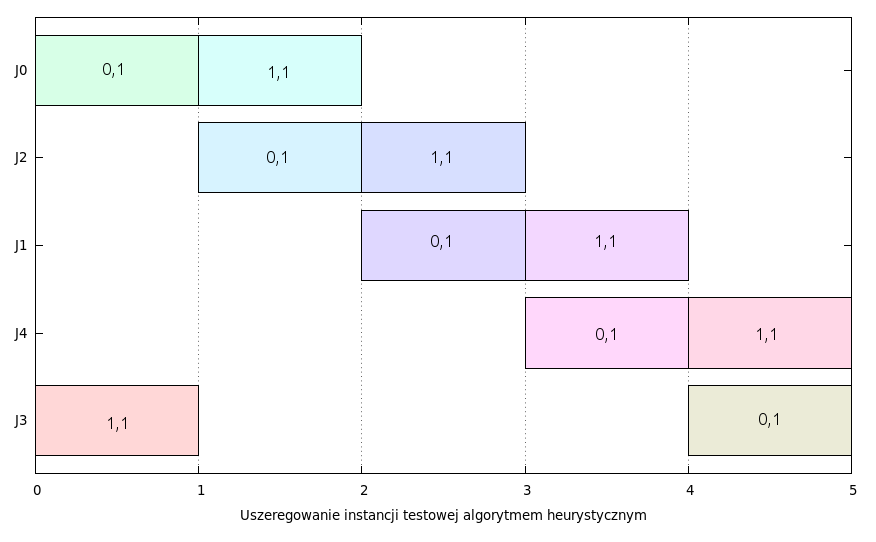
\includegraphics[scale=0.51]{images/gantt.png} \\
\end {center}
\end{figure}

\subsection{Analiza złożoności}
Upraszczając skrajnie powyższy opis algorytmu (Sprowadzając go jedynie do głównych pętli) i zapisując go w składni języka C++ możemy uzyskać następującą postać:\\
\definecolor{darkgreen}{rgb}{0,0.6,0}
\lstset{language=C++,numbers=left,numberstyle=\tiny\color{gray} ,caption={uproszczony zapis kodu na potrzeby analizy złożoności},label=DescriptiveLabel}
\begin{lstlisting}
for(int t = 0; t < m; t++) {
	for(int j = 0; j < n; j++) {
		// uzupelnianie MachineUsage
	}
	for(int i = 0; i < m; i++) { // obliczanie czasow
		/*
			niezaleznie od wielkosci poszczegolnych list
			w tym miejscu wykonanych zostanie _n_ operacji	
			(poniewaz tyle operacji zostalo wrzuconych
			jedna linie wyzej)
		*/
	}
}
\end{lstlisting}
Łatwo zauważyć, iż w ten sposób wykonane zostanie \emph{$O(m \cdot (n + mn)) = O(mn \cdot (m + 1))$} operacji, co daje złożoność kwadratową od ilości maszyn/operacji. Warto pamiętać o tym, iż jest to także kwestia implementacji - uzyskanie takiej złożoności możliwe jest m.in. dzięki zastosowaniu struktur danych typowych dla języka C++; w wypadku innych języków złożoność ta może być większa.
\subsection{Kilka słów o implementacji}
Jak już wspomnieliśmy wcześniej, wykorzystane zostało tu programowanie zorientowane obiektowo, co pozwala na uzyskanie dostępu do wartości charakteryzujących operacje/zadania w czasie liniowym bez zwiększenia narzutu pamięciowego (oraz zwiększa wygodę pisania i czytelność kodu). Zamiast standardowych dynamicznych tablic oraz tworzonych specjalnie na potrzeby projektu list wykorzystane zostały kontenery \emph{std::vector} oraz listy \emph{std::list}. Operacje wejścia/wyjścia odbywają się poprzez strumienie (nagłówek \emph{iostream}), operacje na plikach także przez strumienie (\emph{fstream}) zaś czytanie wartości z plików oraz ich konwersja na liczby przez \emph{sstream}.
\section{Testy}
\subsection{Wprowadzenie}
Kod źródłowy programu wykorzystywanego do testów jak i skrypty powłoki BASH można pobrać tutaj: \url{https://github.com/hun7err/Job-Shop}\\
Przykładowe sposoby użycia skryptów i programu przedstawione zostały na odpowiednich zrzutach ekranu na rysunkach 1-3.

\begin{figure}[!h]
\begin{center}
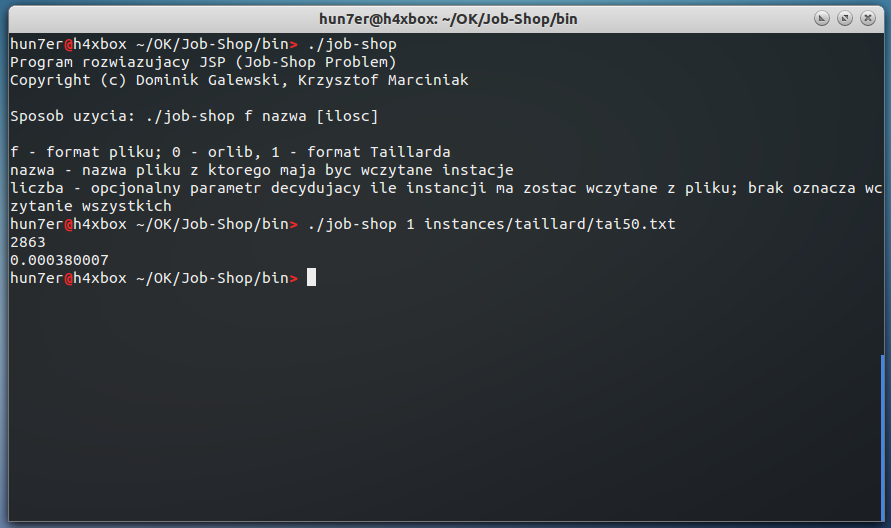
\includegraphics[scale=0.40]{images/uzycie1.png} \\
\end {center}
\caption{Przykładowe użycie programu testowego}
\end{figure}

\begin{figure}[!h]
\begin{center}
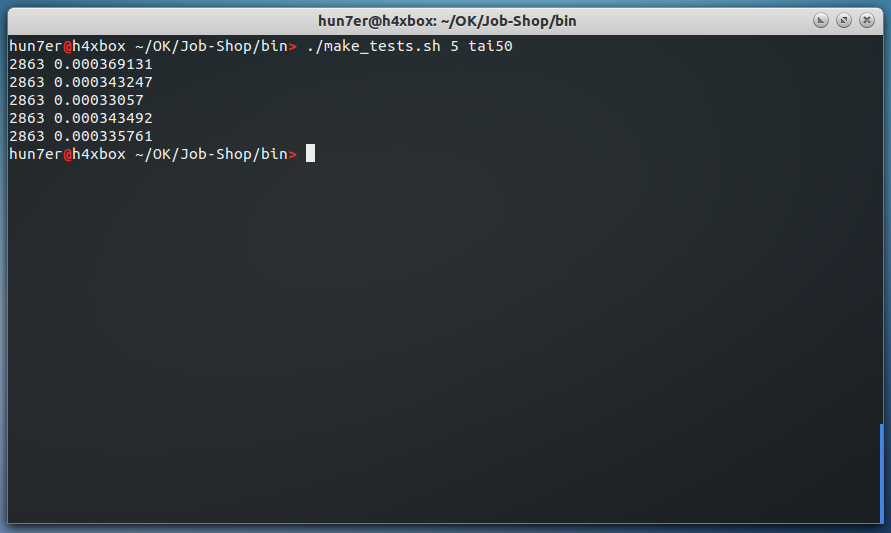
\includegraphics[scale=0.40]{images/uzycie2.png} \\
\end {center}
\caption{Przykładowe użycie skryptu automatyzującego wykonanie programu testowego}
\end{figure}

\begin{figure}[!h]
\begin{center}
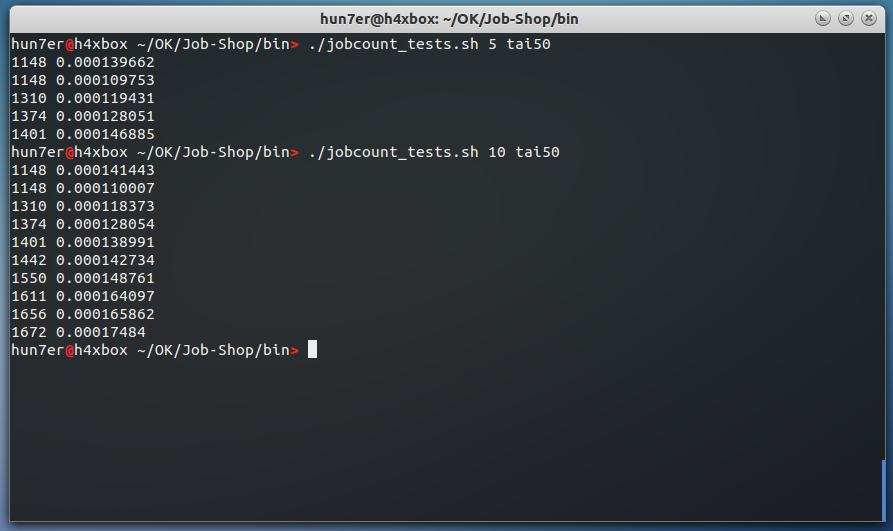
\includegraphics[scale=0.40]{images/uzycie3.png} \\
\end {center}
\caption{Przykładowe użycie skryptu wykonującego n pierwszych zadań instancji}
\end{figure}

We wszystkich przypadkach testowych, aby zminimalizować błąd pomiaru, dokonane zostały serie pomiarów po 5 uruchomień programu testowego każda. Wyniki zamieszczone w sekcji "Wyniki"

\subsection{Wyniki}
Wyniki testów (odpowiednio pomiaru czasu dla instancji Taillarda tai20-24 oraz dodatkowo jakości rozwiązań dla tai25 i czasu dla liczby zadań rosnącej od 1 do 20 przedstawione zostały w tabelach oraz zobrazowane na odpowiednich wykresach zamieszczonych poniżej.


\begin{table}
\begin{center}
\rowcolors{2}{white}{gray!20}
\begin{tabular}{ | c | c | c | c | }
\hline
n & w\_heur & w\_dol & w\_gor \\ \hline
20 & 1937 & 1213 & 1362 \\ \hline
21 & 2312 & 1217 & 1663 \\ \hline
22 & 2283 & 1314 & 1626 \\ \hline
23 & 2196 & 1248 & 1574 \\ \hline
24 & 2233 & 1284 & 1660 \\ \hline
\end{tabular}
\caption{Jakość rozwiązań. Długość uszeregowania dla instancji tai20-tai24: \emph{w\_heur} - długość wygenerowanego uszeregowania, \emph{w\_dol} - długość najkrótszego uszeregowania, \emph{w\_gor} - długość najdłuższego uszeregowania }
\end{center}
\end{table}

\begin{table}
\begin{center}
\rowcolors{2}{white}{gray!20}
\begin{tabular}{ | c | c | c | c | c | c | c | }
\hline
n & pomiar 1 & pomiar 2 & pomiar 3 & pomiar 4 & pomiar 5 & średnia \\ \hline
20 & 0.000249262 & 0.000217277 & 0.000210625 & 0.000372336 & 0.000210778 & 0.0002520556 \\ \hline
21 & 0.000289934 & 0.000259922 & 0.000276765 & 0.000255635 & 0.000254478 & 0.0002673468 \\ \hline
22 & 0.000290523 & 0.000259013 & 0.000277318 & 0.000254619 & 0.000258459 & 0.0002679864 \\ \hline
23 & 0.000293287 & 0.000266415 & 0.000279266 & 0.000260178 & 0.000258515 & 0.0002715322 \\ \hline
24 & 0.000303617 & 0.000259151 & 0.000265288 & 0.000257259 & 0.00025684 & 0.000268431 \\ \hline
\end{tabular}
\caption{Czas wykonywania dla instancji tai20-tai24}
\end{center}
\end{table}

\begin{table}
\begin{center}
\rowcolors{2}{white}{gray!20}
\begin{tabular}{ | c | c | c | c | c | c | c | }
\hline
n & pomiar 1 & pomiar 2 & pomiar 3 & pomiar 4 & pomiar 5 & średnia \\ \hline
1 & 0.000136891 & 0.000138124 & 0.000133193 & 0.000137867 & 0.000132761 & 0.0001357672 \\ \hline
2 & 0.000106611 & 0.000130659 & 0.000112512 & 0.000134897 & 0.000110248 & 0.0001189854 \\ \hline
3 & 0.000118974 & 0.000120523 & 0.000127592 & 0.000119854 & 0.000117705 & 0.0001209296 \\ \hline
4 & 0.000200902 & 0.000125864 & 0.000120298 & 0.000128804 & 0.000124368 & 0.0001400472 \\ \hline
5 & 0.00013748 & 0.000134921 & 0.000131103 & 0.000137612 & 0.000136895 & 0.0001356022 \\ \hline
6 & 0.000144395 & 0.000145004 & 0.000147446 & 0.000148803 & 0.000143128 & 0.0001457552 \\ \hline
7 & 0.000155117 & 0.000148213 & 0.000157253 & 0.000154215 & 0.000153007 & 0.000153561 \\ \hline
8 & 0.000161741 & 0.000162315 & 0.00016641 & 0.000159693 & 0.000163067 & 0.0001626452 \\ \hline
9 & 0.000169827 & 0.000167233 & 0.00018334 & 0.000183315 & 0.00018489 & 0.000177721 \\ \hline
10 & 0.000182562 & 0.000179737 & 0.000175149 & 0.000178495 & 0.000177803 & 0.0001787492 \\ \hline
11 & 0.00020098 & 0.000184428 & 0.000183737 & 0.000183721 & 0.000186297 & 0.0001878326 \\ \hline
12 & 0.000195668 & 0.000200248 & 0.000198276 & 0.000193531 & 0.000195608 & 0.0001966662 \\ \hline
13 & 0.000209934 & 0.000202208 & 0.000217379 & 0.000206239 & 0.000209872 & 0.0002091264 \\ \hline
14 & 0.000205723 & 0.00020741 & 0.000206064 & 0.000211212 & 0.000209396 & 0.000207961 \\ \hline
15 & 0.000218323 & 0.000222152 & 0.000212904 & 0.000215359 & 0.000217206 & 0.0002171888 \\ \hline
16 & 0.000227722 & 0.000222366 & 0.000229543 & 0.000227292 & 0.000223028 & 0.0002259902 \\ \hline
17 & 0.000231938 & 0.00023416 & 0.000237762 & 0.00024043 & 0.000235943 & 0.0002360466 \\ \hline
18 & 0.000246603 & 0.000250798 & 0.000253854 & 0.000238947 & 0.000238493 & 0.000245739 \\ \hline
19 & 0.000254034 & 0.000255494 & 0.000262385 & 0.000252613 & 0.000255069 & 0.000255919 \\ \hline
20 & 0.000256652 & 0.000258174 & 0.000263599 & 0.000273241 & 0.000258198 & 0.0002619728 \\ \hline
\end{tabular}
\caption{Pomiary czasu wykonania dla instancji tai25 z liczbą zadań rosnącą od 1 do 20}
\end{center}
\end{table}


\pagebreak

\begin{figure}[!h]
\begin{center}
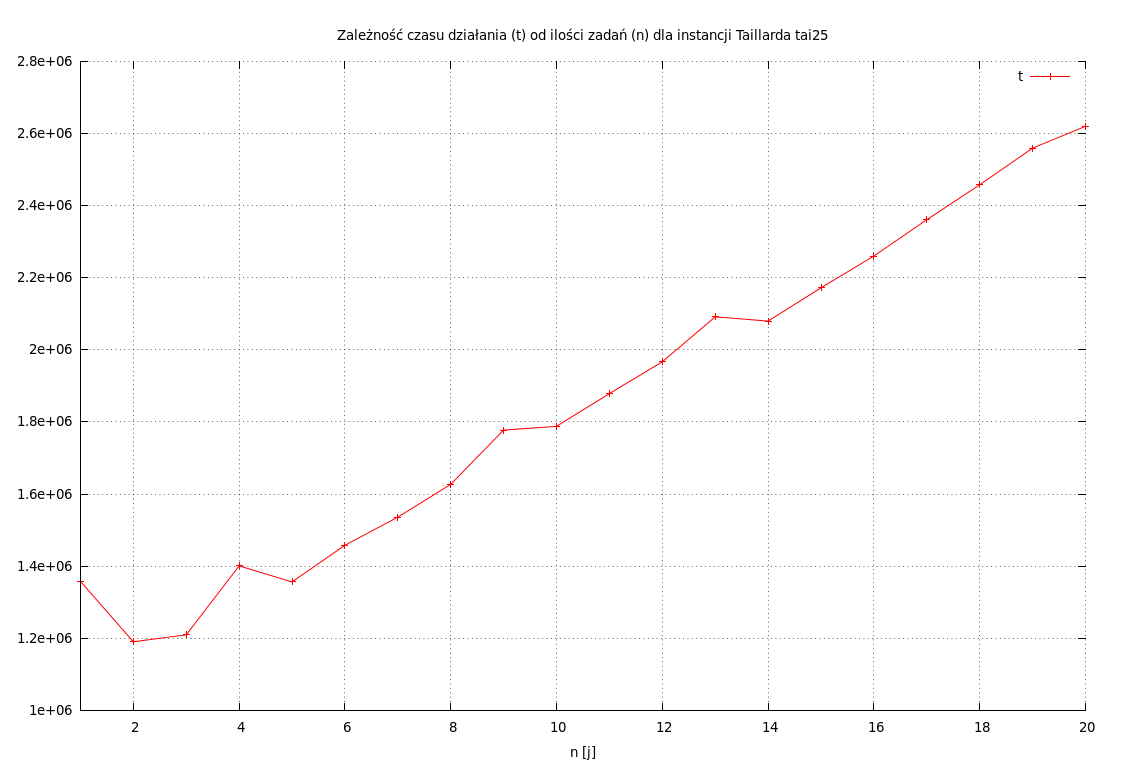
\includegraphics[scale=0.39]{images/wyk1.png} \\
\end {center}
\end{figure}

\pagebreak

\begin{figure}[!h]
\begin{center}
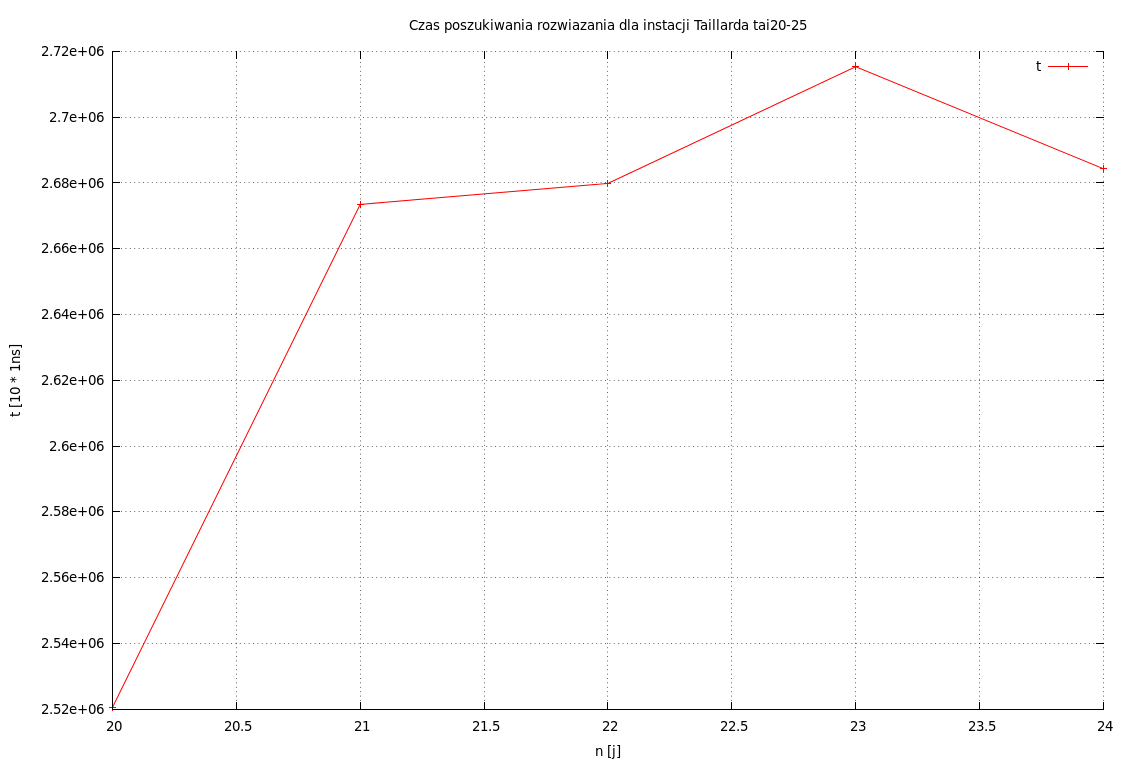
\includegraphics[scale=0.39]{images/wyk2.png} \\
\end {center}
\end{figure}

\begin{figure}[!h]
\begin{center}
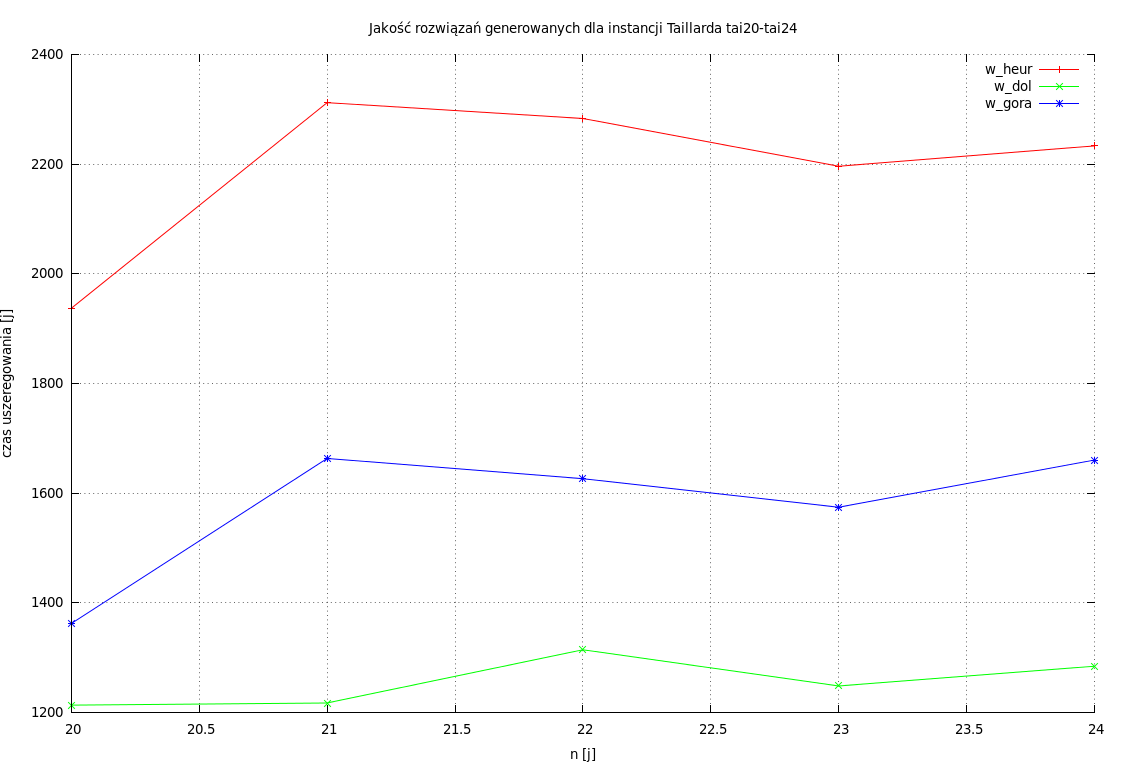
\includegraphics[scale=0.39]{images/wyk3.png} \\
\end {center}
\end{figure}

\pagebreak
\section{Wnioski}
Jak widać po tabelach oraz wykresach generowane wyniki nie są w zadanym przedziale \emph{<w\_dol, w\_gora>} (przynajmniej dla tai25), jednak dla wspomnianej instancji czas uszeregowania tworzy podobną krzywą co \emph{w\_gora}, co pozwala nam sądzić iż wygenerowane rozwiązanie jest dopuszczalne. Algorytm (oraz jego implementacja) zostały sprawdzone dla instancji testowych oraz instancji stworzonych tylko i wyłącznie na potrzeby wyszukiwania potencjalnych błędów, co pozwala sądzić, iż generowane rozwiązania są poprawne.

\end{document}